\chapter{Analisis dan Perancangan}

\section{Analisis Permasalahan}

Pada bagian ini akan dilakukan analisis terhadap hal-hal yang merupakan permasalahan
yang dibahas tugas akhir ini, berupa keadaan pengujian perangkat lunak, BLE,
pengujian keamanan perangkat lunak, dan BDD.

\subsection{Pengujian Perangkat Lunak dan \textit{BLE}}

Menurut kemudahan pengujiannya, kelemahan keamanan terbagi menjadi yang mudah diuji
dan yang sulit diuji. Kelemahan keamanan yang mudah diuji biasanya memiliki penyebab
yang jelas, telah banyak dipelajari, dan memiliki langkah yang mudah untuk mengujinya.
Salah beberapa contoh dari kelemahan ini adalah \emph{Cross Site Scripting} (XSS) dan
\emph{SQL injection}. Kedua kelemahan ini telah banyak dipelajari dan dipahami mekanismenya
sehingga untuk mengujinya telah ada kumpulan \emph{payload} yang bisa digunakan untuk menguji
kelemahan ini. Selanjutnya adalah kelemahan yang sulit diuji. Kelemahan keamanan
yang sulit diuji biasanya belum banyak dipelajari dan membutuhkan penggunaan program
secara normal sehingga tidak bisa langsung diketahui dari awal. Salah satu
dari kelas kelemahan yang termasuk kedalam kelemahan yang sulit diuji adalah
\emph{Business Logic Errors} (BLE).

BLE (CWE-840) merupakan jenis kelemahan yang terjadi karena kekurangan
dan cacat dalam logika bisnis program. Kelemahan BLE biasanya muncul dalam proses bisnis,
alur aplikasi dan urutan langkah-langkah. Jenis kelemahan ini sulit diidentifikasi karena
terjadi sebagai efek samping dari logika bisnis program, bukan karena kelemahan teknologi
yang digunakan, dan sulit diuji karena bentuk nyata dari jenis kelemahan yang terjadi
pada program sebenarnya dapat memiliki banyak bentuk dan untuk menguji kelemahan tersebut
perlu dilakukan urutan langkah-langkah tertentu.

Dalam kebanyakan \textit{Software Development Life Cycle} (SDLC), setelah dilakukan
penggalian kebutuhan, pemodelan arsitektur, dan desain detail akan didapatkan
skenario yang berisi deskripsi-deskripsi fitur yang akan diimplementasikan,
kemudian \emph{programmer} akan mulai melakukan implementasi.
Sementara \emph{tester} akan melakukan
pengumpulan \emph{security requirement} dan \emph{threat modelling} sehingga didapatkan
\emph{misuse case, abuse case} dan \emph{threat model}. Setelah hasil pengumpulan ini
didapatkan, kasus-kasus ini dapat diubah menjadi skenario-skenario yang berisi
langkah-langkah dalam terjadinya suatu kasus ancaman keamanan.

\subsection{\textit{Pengujian Keamanan dengan BDD}}

Dalam BDD, fitur-fitur yang ada dalam sebuah program dideskripsikan dengan skenario
berisi langkah yang menjelaskan alur terjadinya sebuah skenario. Pada kakas BDD
yang ada pada saat ini, biasanya kasus test ini ditulis dengan bahasa dan \emph{syntax}
yang mudah dimengerti semua pihak mulai dari \emph{programmer} yang akan melakukan implementasi
hingga \emph{stakeholder} yang memiliki aplikasi. Penggunaan bahasa tentu saja memiliki \emph{tradeoff}
yang berbentuk dalam sulitnya untuk mendeskripsikan keadaan yang lebih kompleks.

Hasil dari pemodelan ancaman keamanan yang berbentuk skenario yang terdiri dari langkah-langkah
cocok dengan metodologi BDD yang juga mendeskripsikan skenario dari fitur program dalam bentuk
langkah-langkah. \emph{File} fitur BDD berisi pengetahuan tentang kejadian apa saja yang mungkin
terjadi terhadap suatu fitur program. Kumpulan pengetahuan ini dapat digunakan untuk
membantu menemukan kelemahan keamanan yang termasuk kedalam BLE, karena kelemahan BLE
umumnya terjadi setelah langkah-langkah tertentu dijalankan secara berurutan.

Pada saat ini, ada beberapa kakas yang dapat digunakan untuk melakukan metodologi BDD.
Beberapa diantaranya adalah Cucumber dan Rspec.
Cucumber adalah kakas metodologi BDD yang menggunakan bahasa Gherkin. Kakas ini dapat
digunakan dengan beberapa bahasa pemrograman seperti Java, Javascript, Ruby, dan Python.
Sementara Rspec adalah kakas metodologi BDD yang menggunakan DSL Ruby, dan hanya bisa
digunakan dengan bahasa pemrograman Ruby.
Cucumber memiliki kelebihan dimana \emph{file} pengujian ditulis dengan bahasa Gherkin
yang berbentuk bahasa manusia, sehingga dapat dimengerti oleh banyak pihak. Namun kekurangannya
adalah \emph{syntax} Gherkin yang simpel menyebabkan sulitnya untuk mengekspresikan konstruk
yang lebih kompleks karena hanya didesain untuk pengujian fungsionalitas, bukan untuk
pengujian keamanan.

Kerangka kerja pengujian lain yang mirip dengan BDD ada \textit{Test Driven Development} (TDD),
dimana pengujian tetap mengikuti alur yang sama, namun perbedaannya dalam TDD program diuji dalam
tingkat fungsi dalam kode. Kenapa kerangka kerja BDD digunakan dalam penyelesaian masalah ini adalah
karena BLE sendiri terjadi dalam tingkat \textit{business logic} yang diuji oleh BDD, sementara TDD
tidak pada tingkat tersebut.


% \section{============}

% \section{Analisis \emph{Business Logic Error}}

% \subsection{Analisis}

% Celah keamanan bisa terjadi karena pada pada siklus pengembangan perangkat lunak
% biasa, \emph{programmer} hanya fokus terhadap kebutuhan fungsional,
% memerhatikan aspek keamanan. Hal ini juga menjadi penyebab dari BLE.
% BLE, secara spesifik, terjadi karena beberapa hal.
% Pertama, adanya perbedaan kecil dari step sebuah skenario fitur, misal pada state awal,
% jika fitur
% menambahkan barang ke dalam keranjang membutuhkan state awal user untuk telah login,
% apa yang terjadi jika penambahan barang dilakukan saat user belum login.
% Kedua, saat \emph{business} menuliskan deskripsi skenario business logic,
% yang bisa dituliskan dengan mudah biasanya hanya skenario positif dimana
% fitur berjalan sebagaimana seharusnya. Namun, kasus-kasus dimana fitur
% tidak berjalan sesuai dengan seharusnya tidak dituliskan, karena bagi orang bisnis,
% hal itu adalah sesuatu hal yang mereka rasakan \emph{obvious}.
% BLE terjadi saat \emph{programmer} dan \emph{tester} yang tidak memiliki
% pengetahuan domain sebanyak orang bisnis, tidak mengetahun asumsi-asumsi tersebut dan lupa
% untuk mengujinya.

% Dalam masa pengembangan suatu fitur, \emph{programmer} bisa saja memikirkan
% apa saja kemungkinan variasi dari nilai-nilai suatu fitur. Programmer
% dapat mencoba mengakomodasi semua variasi itu, tetapi pengetahuan tentang
% adanya variasi tersebut mungkin hanya teringat pada saat mengerjakan
% fitur tersebut. Sehingga di akhir pada saat melakukan \emph{acceptance test},
% \emph{tester} tidak tau tentang variasi ini dan tidak mengujinya.
% Bahkan, bisa saja \emph{programmer} yang sedang mengerjakan fitur tersebut
% lupa terhadap variasi tersebut beberapa hari kemudian.

% \emph{Tester} bisa saja mencoba memikirkan banyak \emph{abuse case} pada saat
% akan melakukan pengujian suatu fitur, dan tentu menggunakan \emph{tester} yang
% berbeda dengan orang yang melakukan implementasi akan menghilangkan beberapa
% subjektifitas dalam \emph{abuse case}. Namun, sang \emph{programmer} tadi yang
% sempat memikirkan kasus-kasus variasi tentu juga memiliki pengetahuan yang banyak
% tentang fitur tersebut, namun tidak menuliskan kasus-kasus tersebut karena merasa
% melakukan pengujian adalah pekerjaan \emph{tester}, merasa menuliskan kasus pengujian
% adalah hal yang sulit dan hal lainnya seperti di kejar
% deadline, dan lain lain. \emph{Insight} dari \emph{programmer ini} tentu berharga,
% namun tidak terdokumentasi dan hilang.

% \section{Language Requirement}

% Dari analisis di atas kita dapat mengetahui kebutuhan-kebutuhan bahasa
% agar dapat melakukan pengujian efektif terhadap BLE, yaitu:

% \begin{enumerate}
%   % \item Mudah

%   %       Bahasa yang akan dibuat haruslah mudah dipahami, sehingga semua pihak tetap
%   %       bisa memahaminya, dan mudah ditulis, sehingga \emph{programmer} yang ``sibuk''
%   %       terdorong untuk menulis kasus pengujian.

%   \item Bisa menyatakan kegagalan
%   \item Bisa menyatakan variansi

%         Seperti yang telah disebutkan di atas, salah satu penyebab dari BLE adalah
%         adanya variansi-variansi dari skenario.
%         Bahasa yang akan dibuat haruslah dapat menyatakan variansi ini dengan mudah.
%         Hal ini dapat mengurangi duplikasi dan meningkatkan pemahaman bersama.
% \end{enumerate}



\section{Kebutuhan DSL Solusi}

Pada bagian ini akan dibahas tiga poin pengembangan terhadap bahasa Gherkin dan kakas Cucumber
yang dapat diambil untuk membuat Gherkin dan Cucumber menjadi lebih cocok untuk pengujian keamanan.
Tiga poin tersebut adalah kemampuan untuk merepresentasikan kegagalan, kemampuan untuk menyatakan variasi,
dan pengacakan skenario. Dua poin pertama merupakan pengembangan terhadap bahasa Gherkin, dan
poin terakhir merupakan pengembangan terhadap kakas Cucumber sebagai \emph{runtime} bahasa Gherkin.

\subsection{Representasi Kegagalan}

Pada pengujian fungsionalitas, kita hanya menuliskan kasus-kasus positif
dimana skenario berjalan dengan benar. Namun untuk pengujian BLE,
menuliskan dan melakukan pengujian dimana skenario tidak berjalan dengan benar
haruslah sama mudahnya dengan skenario yang benar.

Pada saat ini, penulisan \emph{step} pada Gherkin lebih berorientasi terhadap
kasus sukses. Misalkan untuk step \texttt{Then the basket should have items in it},
dapat memiliki step gagal berupa \texttt{Then the basket should not have items in it}.
Secara semantik hal dua tadi adalah kebalikan, dimana logika pengujian
sama, berbeda namun di akhir kode \emph{step definition}. Hal ini
menyebabkan banyaknya duplikasi kode \emph{step definition} dan membuat \emph{programmer} malas untuk
melakukannya.
Duplikasi ini dikarenakan setiap kode \emph{step definition} dari Gherkin dianggap
sukses/\emph{passing} jika tidak ada exception yang terjadi.
Kita ingin mengurangi duplikasi dan meningkatkan \emph{code reuse}.
Kita ingin agar kode \emph{step definition} dari step \texttt{Then the basket should have items in it}
dapat digunakan untuk skenario sukses ataupun gagal.

Pada saat ini Gherkin hanya menyatakan \textit{step} yang positif seperti
"barang sukses ditambahkan ke dalam keranjang", namun butuh mendeskripsikan \textit{step function}
lagi untuk negatif \textit{step} tersebut seperti "barang gagal ditambahkan ke dalam keranjang" atau
"barang tidak sukses ditambahkan ke dalam keranjang".

Untuk pembahasan fitur ini, kita akan mengacu pada kode Gherkin dibawah:
\begin{lstlisting}[language=gherkin]
Feature: keranjang
  Scenario: menambahkan barang ke dalam keranjang
    Given user telah login
    When user memasukkan 1 barang
    Then ada 1 barang di dalam keranjang
\end{lstlisting}

Untuk desain fitur Failure dapat kita lakukan beberapa hal.

Scenario di atas memiliki initial state dimana user telah login.
Programmer dapat menambahkan satu skenario lagi untuk keadaan dimana user gagal login, seperti:
\begin{lstlisting}[language=gherkin]
Feature: keranjang
  Scenario: menambahkan barang ke dalam keranjang
    Given user telah login
    When user memasukkan 1 barang
    Then sukses ada 1 barang di dalam keranjang
  Scenario: user belum login menambahkan barang 
    Given user belum login
    When user memasukkan 1 barang
    Then gagal ada 1 barang di dalam keranjang
\end{lstlisting}

Fitur \textit{Scenario Outline} dari Gherkin dapat dimanfaatkan untuk memperpendek skenario ini menjadi

\begin{lstlisting}[language=gherkin]
Feature: keranjang
  Scenario Outline: menambahkan barang ke dalam keranjang
    Given user <login state> login
    When user memasukkan 1 barang
    Then <result state> ada 1 barang di dalam keranjang
    Examples:
      | login state | result state |
      | sudah       | sukses       |
      | belum       | gagal        |
\end{lstlisting}

Dengan menggabungkan fitur \emph{scenario outline} dengan \emph{fail scenario}
kita dapat membuat bagian baru dari \emph{scenario outline} yang menyatakan contoh
yang harusnya gagal, sehingga tidak membutuhkan variabel \texttt{result state},
dengan menggunakan fitur tersebut kode pengujian kita dapat menjadi seperti

\begin{lstlisting}[language=gherkin]
Feature: keranjang
  Scenario Outline: menambahkan barang ke dalam keranjang
    Given user <login state> login
    When user memasukkan 1 barang
    Then ada 1 barang di dalam keranjang
    Examples:
    | login state   |
    | telah         |
    Fail Examples:
    | login state   |
    | belum         |
\end{lstlisting}

Sebagai kesimpulan, pada bagian ini diperlukan penambahan jenis skenario \emph{Fail Scenario}
dengan bentuk yang mirip skenario biasa seperti

\begin{lstlisting}[language=gherkin]
Fail Scenario: scenario desc
  (steps...)
\end{lstlisting}

dan menambahkan tabel data baru ke \emph{scenario outline} seperti

\begin{lstlisting}[language=gherkin]
Scenario Outline: menambahkan barang ke dalam keranjang
  (steps...)
  Fail Examples:
    (table...)
\end{lstlisting}



\subsection{Kemampuan Menyatakan Variansi}

Gherkin pada saat ini memiliki fitur \emph{scenario outline} yang dapat menyatakan banyak skenario yang mirip
hanya dalam satu skenario saja dengan menggunakan template dan tabel.
\emph{Scenario outline} dapat memenuhi kebutuhan bahasa untuk menyatakan variansi.

Namun fitur ini dapat dikembangkan dengan menambah kemampuan untuk menyatakan domain/tipe data suatu variabel, misalkan
domain \texttt{integer}, \texttt{positive}, \texttt{string}, \emph{enum}, dan lain lainnya.
Hal ini membuat deklarasi variansi lebih singkat dan padat.
Kemampuan ini juga dapat digabungkan dengan poin sebelumnya.
Untuk \emph{Scenario outline}, kita dapat menyatakan tabel \emph{example} dengan
kombinasi-kombinasi varian yang harus gagal.
Untuk domain variabel, kita dapat menyatakan nilai mana saja yang harus gagal.

Sebagai contoh dalam aplikasi \emph{e-commerce}, seorang user dapat memiliki status
telah atau belum \emph{login}. Seperti yang telah dibahas pada poin sebelumnya, kita dapat
menggunakan fitur \emph{scenario outline} dan \emph{fail scenario} untuk menyatakan
pengujian fitur tersebut. Namun dengan bertambahnya fitur dan skenario yang akan diuji,
mengulang penggunaan \emph{scenario outline} yang berulang-ulang menjadi sulit. Dengan contoh
di atas tentu saja \emph{state} seorang user simpel saja, hanya sudah atau belum login, namun
jika atribut yang dimiliki user memiliki banyak nilai, misalnya jenis user yang dapat
berupa admin, pembeli dan penjual, jika ada perubahan dari spesifikasi maka semua tempat
yang terkait dengan atribut ini harus diubah.

Untuk mengatasi hal ini, kita dapat menambahkan fitur dimana kita dapat membuat deklarasi
nilai-nilai yang dapat dimiliki suatu variabel, seperti enum. Sebagai contoh, fitur admin
dashboard suatu aplikasi \emph{e-commerce} dapat diuji dengan menggunakan kode berikut

\begin{lstlisting}[language=gherkin]
Variables:
  user role: enum buyer, seller, admin
Feature: Admin
  Scenario: admin mengubah setting website
    Given user dengan role <user role> telah login
    When user merubah pengaturan website
    Then pengaturan website berubah
    Variables Accepted:
    | user role    |
    | admin        |
\end{lstlisting}

Bagian pada \texttt{Variables Accepted} mirip dengan bagian \emph{Examples} pada
scenario outline, namun \emph{tester} hanya perlu menulis kombinasi nilai variabel-variabel
yang diterima, \emph{runtime} gherkin akan secara otomatis menguji semua kombinasi variabel.

Deklarasi ini bersifat global sehingga dapat digunakan di file fitur lainnya.
Dengan fitur ini duplikasi di dalam kode pengujian menjadi berkurang dan
kode memiliki satu sumber fakta sehingga jika terjadi perubahan pada spesifikai tidak
harus mengubah kode pada banyak tempat.

Untuk bagian ini, pada gherkin akan ditambahkan bagian \emph{Variables} yang digunakan
untuk deklarasi variabel. Bagian ini akan terletak pada tingkat yang sama dengan bagian \emph{Feature}
dan berbentuk seperti

\begin{lstlisting}[language=gherkin]
Variables:
  (nama variabel 1): enum (values 1...)
  (nama variabel 2): enum (values 2...)
  ...
\end{lstlisting}

Untuk menggunakan deklarasi ini melalui table \emph{Variable Accepted} dan/atau \emph{Variable Rejected}
yang dapat digunakan di bagian \emph{scenario} atau \emph{fail scenario} seperti

\begin{lstlisting}[language=gherkin]
Scenario: scenario description
  (steps...)
  Variable Accepted:
    (table...)
  Variable Rejected:
    (table...)
\end{lstlisting}

\subsection{Pengacakan Skenario}
\label{sec:323}

Salah satu penyebab kesulitan dari pengujian kelemahan keamanan jenis BLE adalah karena kelemahan
ini memiliki langkah-langkah yang harus dijalankan di dalam aplikasi, namun teknologi pada saat
ini masih belum bisa melakukan eksplorasi langkah-langkah yang bisa dilakukan dalam aplikasi
dari satu \emph{state} ke \emph{state} lainnya, terutama dalam aplikasi berbasis web.

Dalam \emph{file} pengujian BDD telah terdapat sekumpulan pengetahuan tentang langkah-langkah
yang dapat terjadi dalam suatu aplikasi dalam bentuk \emph{step} given, when dan then.
Pengetahuan ini dapat dimanfaatkan oleh kakas pengujian untuk membangkitkan skenario-skenario
baru secara acak dengan harapan skenario acak ini dapat membantu menemukan kelemahan-kelemahan baru.
Cara ini mirip dengan \emph{fuzzy testing} dimana kasus pengujian dibangkitkan secara acak.

Untuk bagian ini, pada \textit{runner} gherkin akan ditambahkan fitur pembangkitan skenario acak
yang diambil dari step-step yang ada dalam skenario-skenario pengujian. Setelah skenario baru ini
dibangkitkan kemudian akan dilakukan pengujian seperti biasa. Hasil dari pengujian skenario acak
ini akan kemudian dilaporkan kepada user.

Dalam bentuk psudeocode python, pengujian ini dapat digambarkan sebagai berikut.


\begin{lstlisting}[language=python]
def all_features
def all_steps = get_all_step_from(all features)

def generate_random_scenario():
  step_amount = randint

  result_scenario = Scenario()

  for _ in range step_amount:
    step = a random step in all_steps
    result_scenario add step

  return result_scenario
\end{lstlisting}

\section{Rancangan Solusi}
\subsection{Struktur Bahasa}
\label{sec:struktur-bahasa}

Pada bagian ini akan dipaparkan grammar bahasa yang akan dibuat dalam \emph{Extenden Backus-Naur Form}(EBNF).
EBNF adalah bahasa simpel yang digunakan untuk mendeskripsikan \emph{grammar} dan \emph{syntax}.
Dalam EBNF, bahasa dideskripsikan menggunakan terminal dan non-terminal.
Terminal adalah simbol yang berupa teks sebenarnya yang akan tampak pada kode program,
pada contoh dibawah terminal akan ditandai dengan menggunakan tanda kutip.
Non-terminal adalah kumpulan dari terminal dan non-terminal lainnya yang menentukan struktur dari
program. Non-terminal selain dibuat dari terminal dan non-terminal lainnya juga dapat menggunakan
simbol yang biasa digunakan pada regex seperti \texttt{.+*|}.

Gherkin yang menggunakan bahasa manusia memiliki struktur yang cukup bebas
namun kita masih dapat memperkirakan grammarnya dalam EBNF.

\begin{lstlisting}[language=ebnf]
string
  : .+ ;
token
  : \w+ ;
newline
  : \n ;
stepKeyword
  : 'given' | 'when' | 'then' ;
stepLine
  : stepKeyword string newline ;
stepLines
  : stepLine+ ;
scenarioKeyword
  : 'scenario' | 'fail scenario' ;
scenario
  : scenarioKeyword ':' string newline
    stepLines variableAcceptedTable?;
backgroundScenario
  : 'background' ':' string newline stepLines ;

tableLine
  : '|' ( string '|' )+ ;
dataTable
  : (tableLine newline)+ ;
dataTableBody
  : ':' newline dataTable ;
exampleDataTable
  : ('example' dataTableBody)? ('fail example' dataTableBody)? ;
scenarioOutline
  : 'scenario outline' ':' newline stepLines
    exampleDataTable? variableAcceptedTable?;

variableDeclarationType
  : 'enum' string (',' string)*
  | 'bool' ;
variableDeclarationEntry
  : string ':' variableDeclarationEntry newline ;
variableDeclaration
  : 'variable' ':' newline variableDeclarationEntry+ ;
variableAcceptedTable
  : 'variable accepted' dataTableBody ;

featureChild
  : scenario | backgroundScenario
  | variableDeclaration | scenarioOutline ;
feature
  : 'feature' ':' string newline featureChild+;

topLevelEntry
  : feature | variableDeclaration ;

featureFile
  : topLevelEntry+ ;
\end{lstlisting}

Dari grammar EBNF di atas, penambahan grammar untuk poin representasi kegagalan terdapat pada baris 14 dan 28,
dan untuk poin kemampuan menyatakan kegagalan terdapat pada baris 31-41, 45, dan 50.

\subsection{Pengacakan Skenario}

Salah satu fitur tambahan pada gherkin yang direncanakan adalah fitur pengacakan skenario.
Untuk pembangkitan skenario acak ini tentu tidak bisa hanya asal acak, karena tidak akan menghasilkan
skenario pengujian yang efektif, seperti skenario acak yang dihasilkan tidak memiliki satupun step \texttt{Then}
sehingga tidak dilakukan \textit{assertion} terhadap hasil eksekusi skenario dan menghasilkan \textit{false positive}.
Selain syarat di atas tidak menutup kemungkinan adanya syarat-syarat lain yang perlu diikuti namun saat ini masih belum
diketahui.
Kakas juga tidak dapat memastikan bahwa skenario yang dibangkitkan terlepas dari \textit{false positive} atau
\textit{false negative} karena kakas tentu tidak bisa memahami apa yang dilakukannya.

\section{Arsitektur Sistem}

Dalam pembuatan kakas ini, ada tiga komponen yang saling bekerjasama. Pertama adalah \emph{parser} yang
berfungsi untuk mengubah \emph{file} fitur menjadi struktur data yang lebih mudah diolah. Kedua adalah
\emph{importer} yang berfungsi untuk membaca \emph{file} python dan mengumpulkan seluruh definisi step.
Ketiga adalah \emph{runtime} yang menerima hasil dari \emph{parser} dan \emph{importer} dan kemudian
menjalankan pengujian. Diagram arsitektur seperti pada gambar \ref{dia:desain-arsitektur}.

\begin{figure}[h]
  \centering
  % 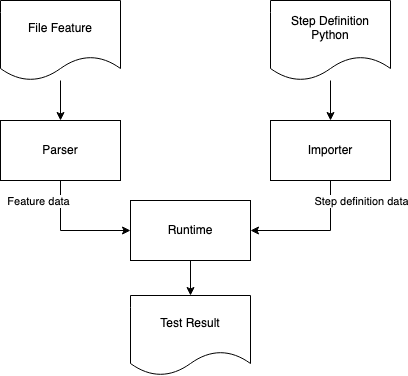
\includegraphics[width=0.8\textwidth]{resources/desain-arsitektur.png}
  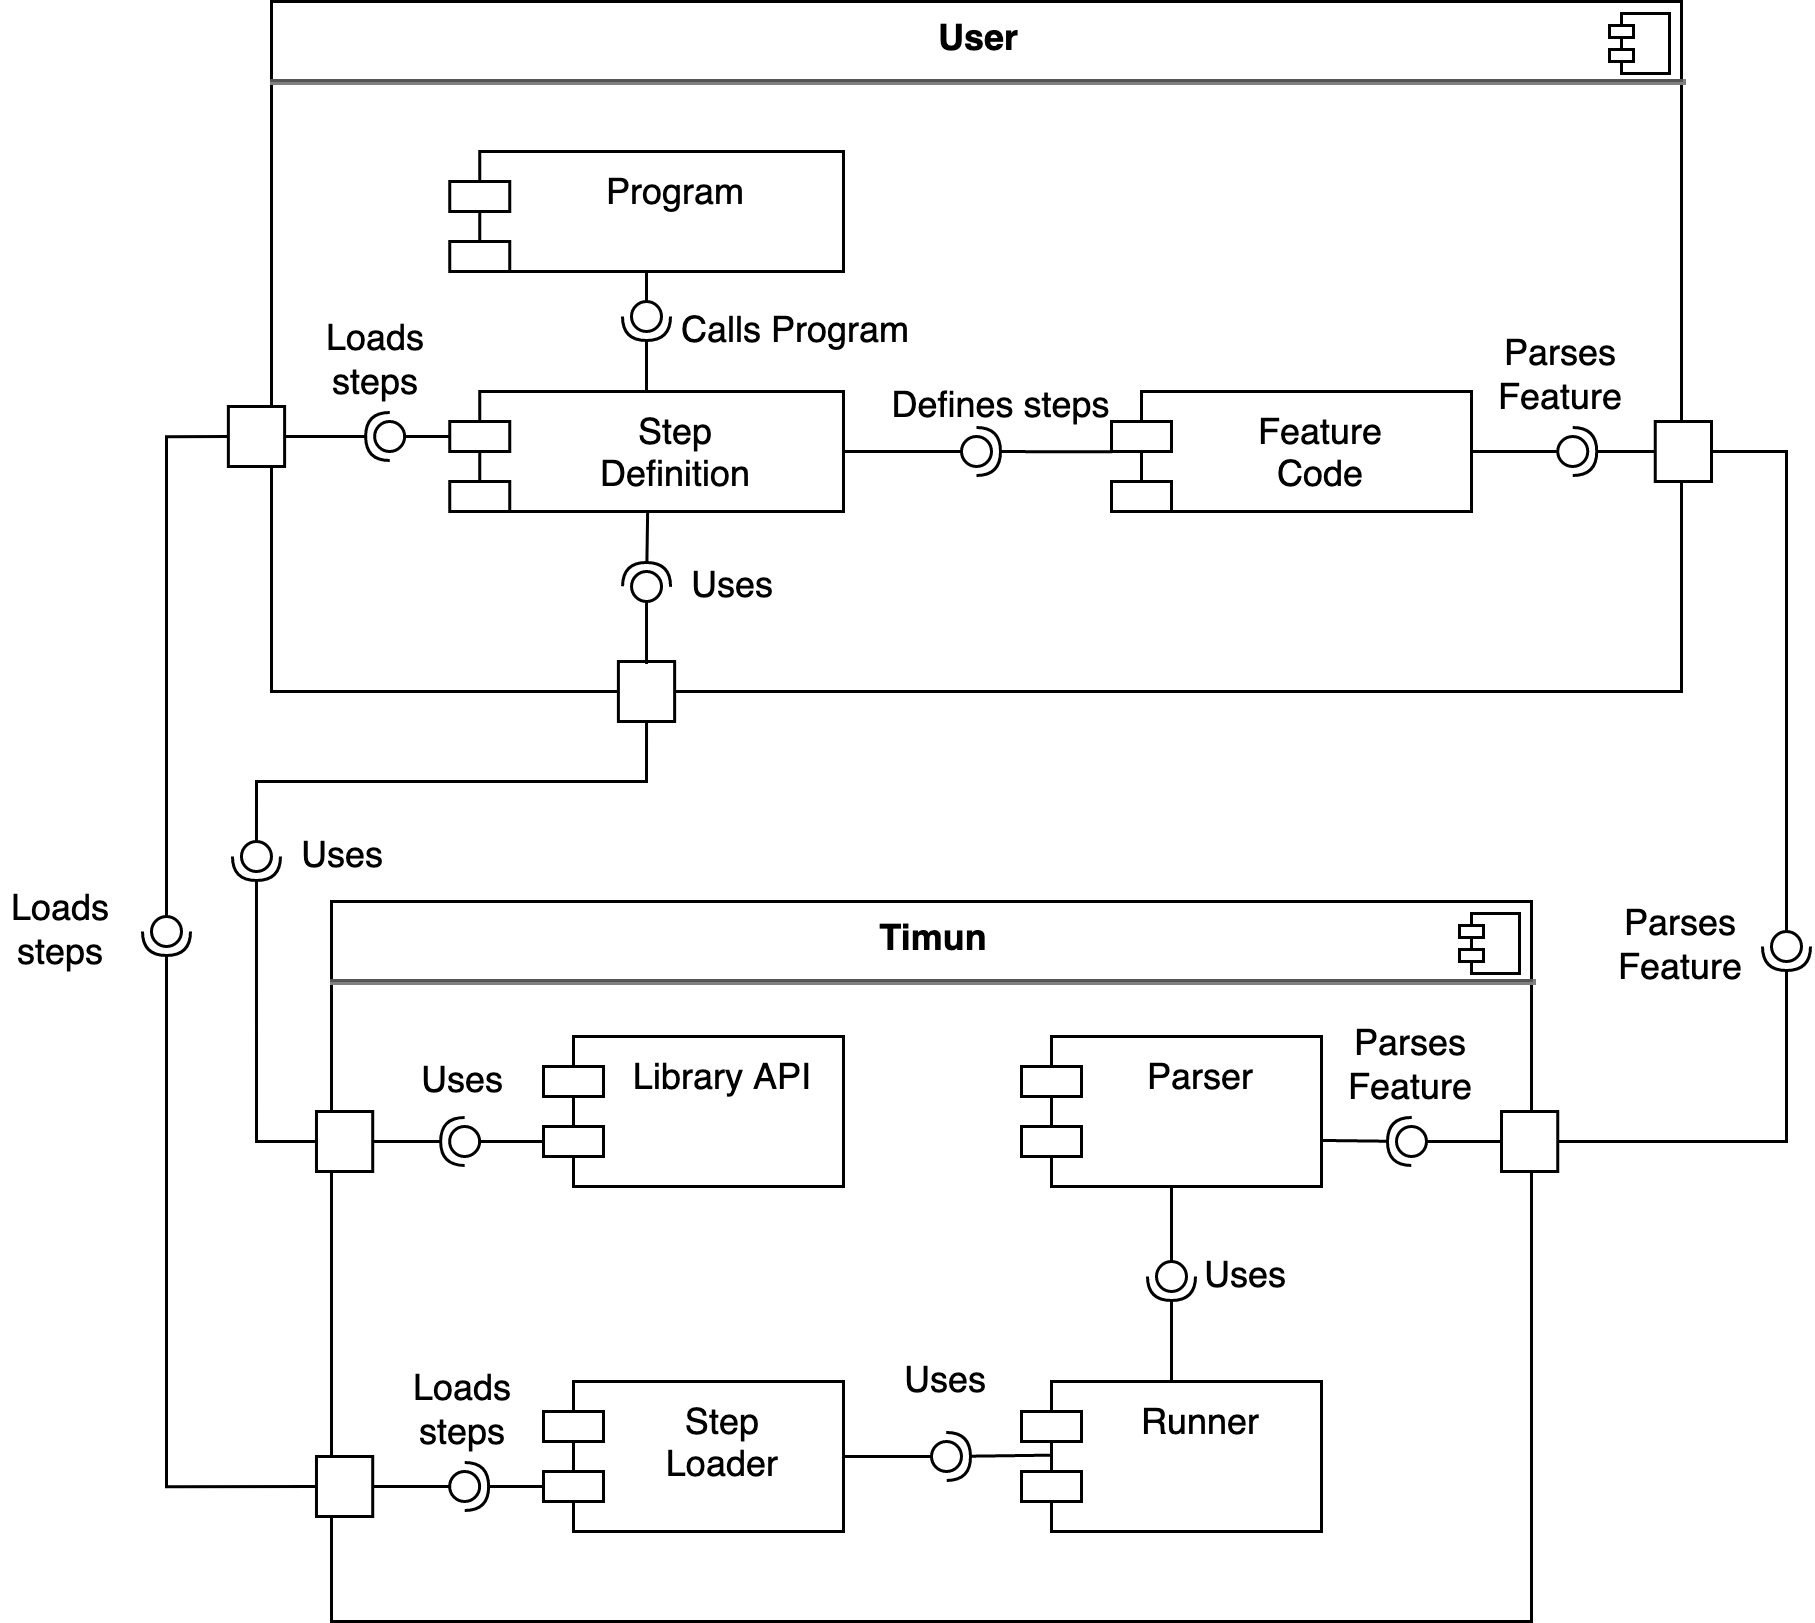
\includegraphics[width=1\textwidth]{resources/component.png}
  \caption{Desain Arsitektur Kakas}
  \label{dia:desain-arsitektur}
\end{figure}

Modul \texttt{User} mengilustrasikan bagian yang harus dibuat oleh user yang akan menggunakan kakas ini,
sementara modul \texttt{Timun} adalah kakas yang digunakan untuk pengujian program.

Pada tugas akhir ini bagian yang akan diimplementasikan terdapat di dalam modul \texttt{Timun}.
Bagian ini terdiri dari 4 komponen. Semua komponen akan diimplementasikan dari awal,
dengan Gherkin dan Cucumber sebagai referensi dan inspirasi untuk implementasi.

% \section{Rancangan Solusi}

% Dari bagian sebelumnya, pada bagian ini akan dibahas desain bahasa untuk fitur yang dianalisa
% dan cara implementasi.

% \subsection{Menyatakan Kegagalan}


% \subsubsection{Variansi}

% Pada bagian sebelumnya telah

% \section{Perbedaan Pengujian Fungsionalitas dan \emph{Business Logic Error}}

% Pengujian untuk fungsionalitas dan untuk keamanan memiliki perbedaan. 
% Pada pengujian fungsionalitas, yang dibutuhkan hanyalah untuk menguji apakah
% fungsionalitas telah terimplementasikan dengan benar.
% Namun pada pengembangan aplikasi terkadang secara tidak sengaja ada fungsionalitas
% tambahan yang bisa menjadi celah keamanan yang sering terlupakan untuk diuji.
% Salah satu macam dari celah ini adalah \emph{business logic error}.

% Pengujian untuk \emph{business logic error} dilakukan dengan memperhatikan tiap-tiap fungsionalitas
% yang diimplementasikan dalam program dan menguji kemungkinan variasi keadaan pada
% fungsionalitas tersebut. Salah satu contohnya adalah pada aplikasi \emph{e-commerce} yang memiliki
% fitur keranjang. Pada fungsionalitas "bisa menambahkan barang ke dalam keranjang", dapat memiliki
% prasyarat bahwa user hanya bisa memasukkan barang ke dalam keranjang jika sudah login, dan skenario
% ini lah yang biasa diuji pada pengujian fungsionalitasnya. Namun untuk \emph{business logic error} 
% terjadi saat asumsi-asumsi normal itu tidak berlaku seperti, bagaimana jika user belum login,
% bagaimana jika user memasukkan -1 barang, dan lain-lain.

% Salah satu cara pengujian fungsional dapat diintegrasikan ke dalam siklus pengembangan aplikasi
% adalah dengan menggunakan kerangka pengujian BDD atau TDD. Kerangka ini mengharuskan \emph{programmer}
% untuk menulis spesifikasi dan kasus uji sebelum mulai menulis kode.
% Salah satu dari kerangka ini adalah Cucumber BDD, beserta bahasa yang ia gunakan untuk mendeskripsikan
% kasus uji, yaitu Gherkin.

% Gherkin adalah bahasa yang digunakan untuk mendeskripsikan spesifikasi fungsionalitas
% aplikasi. Spesifikasi ini ditulis per-skenario, dimana tiap-tiap skenario dibagi menjadi
% langkah-langkah simpel yang menjelaskan skenario tersebut. Dari Gherkin ini kemudian
% digunakan oleh Cucumber untuk menjalankan pengujian.

% Gherkin jika digunakan dengan baik dapat membantu implementasi dan
% pengujian fungsionalitas aplikasi. Tetapi, Gherkin masih belum bisa digunakan untuk melakukan
% pengujian \emph{business logic error} dengan mudah.
% Dalam siklus pengembangan perangkat lunak, \emph{programmer} biasanya memiliki
% banyak deadline yang harus dikejar, sehingga pengembangan hanya seperti ``kejar tayang'',
% yang menyebabkan \emph{programmer} hanya memperhatikan sisi fungsionalitas dari perangkat lunak.
% Adanya kesulitan dalam melakukan pengujian keamanan dapat membuat
% \emph{programmer} semakin enggan melakukannya, walaupun mungkin pada saat
% melakukan rancangan solusi dan implementasi \emph{programmer} juga memikirkan kemungkinan
% kesalahan atau celah keamanan yang mungin terjadi.
% Jika kesulitan-kesulitan tersebut dapat dihilangkan maka \emph{programmer} akan
% dapat langsung menuliskan kasus-kasus pengujian keamanan.
% Namun ada dua hal yang dapat ditambahkan
% ke dalam Gherkin untuk mempermudah pengujian \emph{business logic error}, yaitu kemampuan untuk
% mengecek kegagalan, dan kemampuan untuk mendefinisikan banyak state/value dengan mudah.

% \section{Failure}

% Kekurangan pertama Gherkin yang akan dibahas adalah ketidakmampuan untuk
% menyatakan suatu skenario harus gagal.
% Hal ini terjadi karena desain Gherkin yang bertujuan untuk menguji fungsionalitas saja,
% sehingga setiap step Gherkin dianggap benar jika tidak ada \emph{error}/\emph{exception}
% dari fungsi implementasi stepnya.
% Namun untuk pengujian \emph{business logic error}, dibutuhkan kemampuan untuk menyatakan
% bahwa suatu skenario atau stepnya harus gagal, dan pengujian dianggap tidak lolos
% jika skenario tersebut tidak gagal (dalam bentuk \emph{error/exception}).

% Dengan kemampuan untuk mendefinisikan bahwa suatu skenario harus gagal,
% \emph{programmer} dimudahkan untuk membuat lebih banyak test case
% yang menguji keamanan \emph{business logic error}.
% Pada saat ini pengujian kasus yang harus gagal bisa dilakukan
% pada Gherkin, namun dengan mendefinisikan suatu \emph{step} sebagai negatif.
% Hal ini dapat menyebabkan banyak duplikasi kode-kode yang pada dasarnya
% melakukan hal yang sama.

% \section{Variable Domain}

% Pada saat ini, Gherkin memiliki fitur \emph{scenario outline}
% untuk mendefinisikan sebuah \emph{template} skenario,
% di dalamnya dapat digunakan \emph{placeholder} variabel yang dapat didefinisikan
% dalam sebuah tabel.
% Penggunakan \emph{scenario outline} memungkinkan \emph{programmer} untuk
% mendefinisikan banyak skenario yang mirip dengan variasi nilai dengan mudah.

% Fitur ini dapat dikembangkan dengan menambahkan fungsionalitas dimana 
% variabel-variabel yang digunakan dapat diberikan tipe data,
% sehingga memiliki domain yang jelas. Tipe data dapat berupa \emph{enum string},
% \emph{integer}, \emph{positive integer}, dan lain lain.
% Fitur ini digabungkan dengan kemampuan untuk menyatakan
% skenario yang harus gagal dapat mempermudah \emph{programmer}
% dalam mendeskripsikan kasus-kasus pengujian keamanan bersamaan dengan
% menulis kasus pengujian fungsionalitas.